\subsection{Word Salience}

\begin{frame}{Deep Learning Models of Word Salience}


 
\textbf{Goal:} Make lexical information more useful for DL models of 
sentence extractive summarization.\\
~\\
\textbf{Why?} 
\begin{itemize}
 \item Improve explanation.
 \item Improve generalizability I (to Multi-Doc)
 \item Improve generalizability II (to Abstractive Summarization)
\end{itemize}
\end{frame}

\begin{frame}{Word Features}

    \begin{itemize}
        \item Feature Embeddings
        \begin{itemize}
        \item Shallow lexical semantics (Glove Embeddings)
        \item Term Frequency 
        \item Topic Signature 
        \item POS tag
        \item Named-Entity tag
        \item Dependency role
        \item Dependency depth (distance from root node)
        \item LDA Topic/Brown Cluster 
        \end{itemize}
~\\
        \item Contextualized representation (Elmo Embeddings)
    \end{itemize}


\end{frame}

\begin{frame}{Proposed Model}
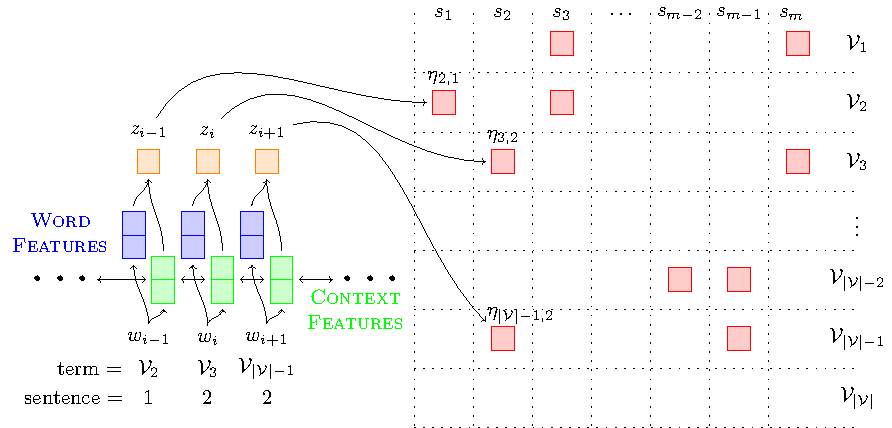
\includegraphics[scale=.6]{images/section3/4_2_wimp_model.pdf}

    $\omega \triangleq $ Sentence $\times$ Term matrix of word salience 
    weights, e.g. $\omega_{i,j}$ is the importance score of term $j$ 
    in sentence $i$ \\
%~\\
%$\omega_{i,j} = \sum 1_{i,j,t}  z_t$ \\
%~\\
%$1_{i,j,t}$ is 1 if the $t$-th word in the document occurs in sentence $i$ and is equal to the $j$th term in the vocabulary.




\end{frame}

\begin{frame}{Proposed Experiments}
\begin{itemize}
   \item Learn word importance scores on large news datasets (CNN/DM, NYT, Newsroom, XSUM)
    \item Many ways to construct a summary from $\omega$.
    \item To start, greedy maximization of sum of importance scores, and
    \item large margin learning frame work.

\end{itemize}
\end{frame}

\begin{frame}{Large Margin Learning}

    $\omega \triangleq $ Sentence $\times$ Term matrix of word salience 
    weights, e.g. $\omega_{i,j}$ is the importance score of term $j$ 
    in sentence $i$ \\

    ~\\
    $y \in \mathbb{Z}^n$ is an extractive reference summary of $n$ sentences.
    ~\\
    ~\\
    $\eta \triangleq \sum_{j \in \{1, \ldots, |\mathcal{V}|\}} 
        \max_{i \in y} \omega_{i,j},$ the score for the reference summary.
    ~\\
    ~\\
    $\hat{y}, \hat{\eta}$ predicted summary indices and score.
    ~\\
    ~\\
    $\mathcal{L}(y, \hat{y}) = \max\left(0, 1 + \hat{\eta} - \eta \right) $ 
    ~\\
    ~\\
%    Auxiliary objective: $\mathcal{L}_{word}(z, \zeta) = -\sum_t \zeta_t \log z_t + (1 - \zeta_t) \log 1 - z_t  $ \\
%   where $\zeta_t = 1$ if the $t$th input word occurs in the reference abstract
%summary and 0 otherwise.

\end{frame}

\begin{frame}{Other experiments/Plan B's}

    \begin{itemize}
        \item We can supervise the individual importance scores using
            the reference abstracts to get labels, i.e. $z_i \rightarrow 1$
            if $w_i$ occurs in the reference summary.
            ~\\~\\
        \item More sophisticated inference, e.g. knapsack packing.~\\~\\
        \item Matching performance of sentence extractive models ok if 
            word level scores gives additional explanability.
            ~\\~\\
        \item We can experiment with selective word class masking for 
            domain adaptation, i.e. train Adj./Adv. 
            only model (with no position)
            on news and evaluate on Reddit.)
    \end{itemize}
\end{frame}



\begin{frame}{Generalize to multi-document summarization}
\begin{enumerate}
\item For each document $d \in \{1, \ldots, D\}$ create word importance 
scores  $z_1^{(d)}, \ldots, z_{m_d}^{(d)}$.
\item Compute document set level attention matrix 
    $\Lambda \in \mathbb{R}^{M \times M}$ where $M = \sum_d^D m_d$ and 
\[ \Lambda_{i,j} = \sigma(h_i^Th_j / \tau + b)   \] and $h_i$ are outputs
 of the contextual representation of the $i$-th word (e.g. ELMO embedding).
\item Compute aggregate importance scores $\bar{z_i} = \sum_{j=1}^M z_j \cdot \Lambda_{i, j}$ 
\item Create $\omega$ for all sentences in the document set using the aggregated scores  $\bar{z}_i$. 
\item Proceed as in the single-document summarization model.
\end{enumerate}
\end{frame}

\begin{frame}{Supervise Attention for Abstractive Summarization}

    \begin{itemize}
        \item Normalized importance scores $z_i$ form a distribution over 
            input tokens, like attention.
        \item This could be used in a couple ways:
            \begin{itemize}
                \item Attention could be supervised to match the importance
                    scores, i.e. supervising the content selection in the 
                    decoder.
                \item Directly masking the input to the decoder.
            \end{itemize}
    \end{itemize}

\end{frame}
